\chapter[Chapter 3: Research Methodology]{Research Methodology}

\section{Background}

We will use a mixed method study in order to gain a complete understanding of the \gls{cita} on \gls{chip} system. Quantitative analysis will be used to find trends in student grades between classrooms that do and do not use the program. In parallel, we will conduct a qualitative study to determine student reactions to the program and how they feel their learning was affected. A breakdown of our methodology is shown in Figure \ref{fig:flowchart}.

\begin{figure}[!htb]
	\centering
	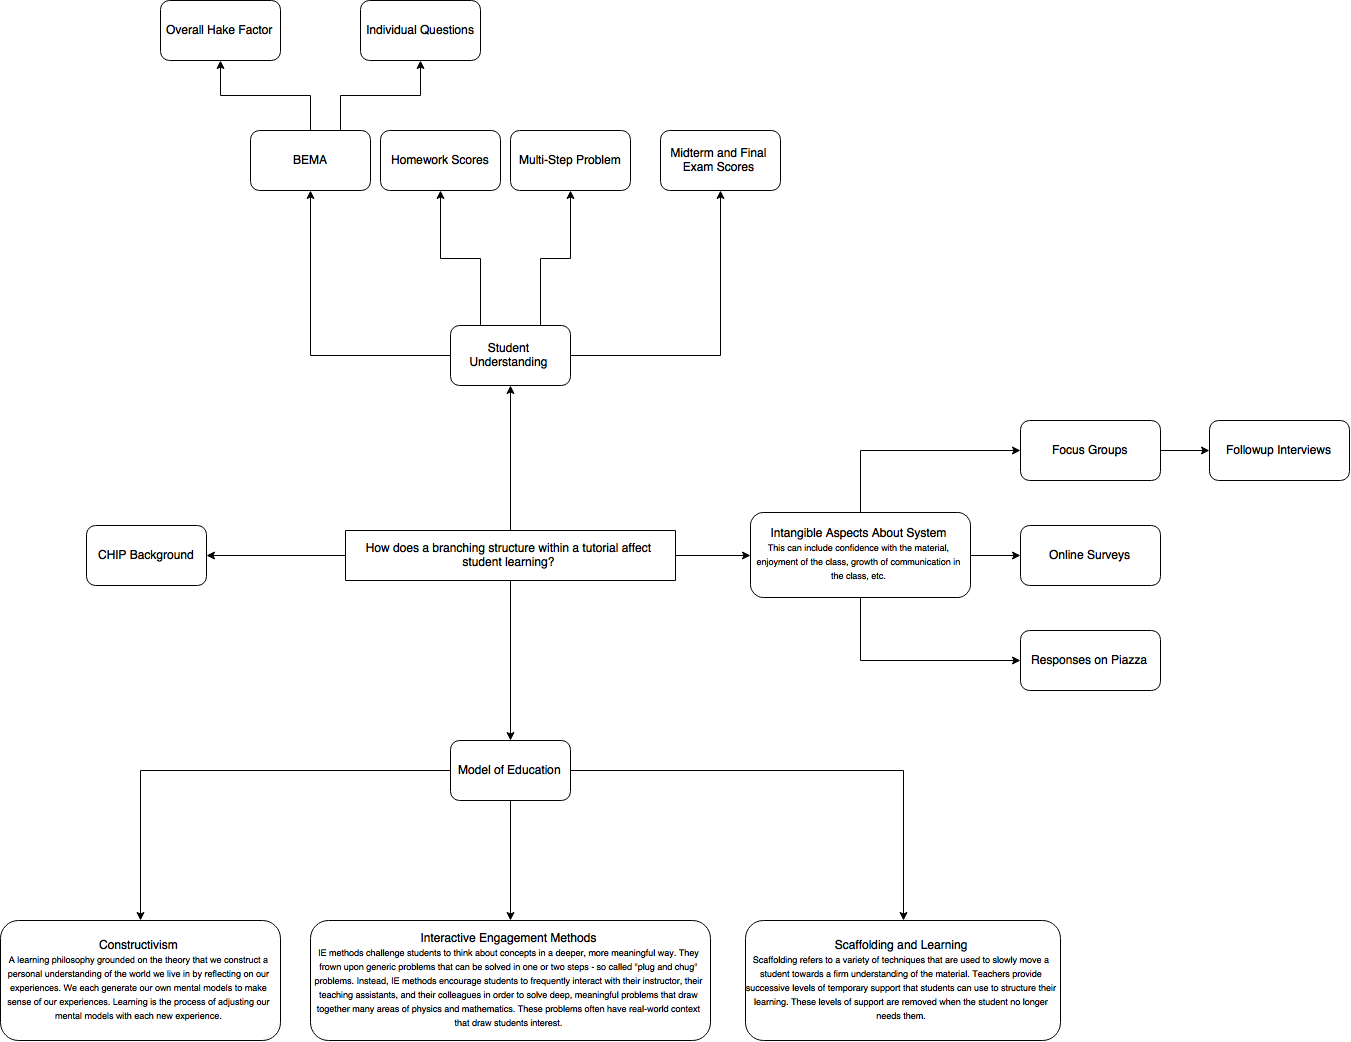
\includegraphics[width=6in]{img/chapter3/flowchart}
	\caption[Flowchart]{Flowchart}
  \label{fig:flowchart}
\end{figure}

\section{General Information About Student Population}

The population that we are studying is engineering and science

The combined yearly enrollment of PHYS 24100 and PHYS 24100D has an average of about 1500 students from science and engineering. Additionally, we have seen an increase in the number of students in online sections ever since the distance learning course was started in the summer semester of 2012.

\section{Quantitative Inquiry}

\section{Exams and Quizzes}



\section{Homework}

The ultimate test of \gls{cita} on \gls{chip} is the ability to solve problems on exams. Student
performance on exam problems that are similar to \gls{cita} enhanced problems will be used to
determine if \gls{cita} improved learning outcomes, i.e. whether or not students have learned
specific problem solving strategies. We can correlate exam scores with:
• Which students use \gls{cita} (“A” students or students at all grade levels)
• When students started using \gls{cita} (before or after first exam, first homework, etc.)
• How many attempts on a problem are made before using \gls{cita}
• How many attempts to solve a problem are needed after using \gls{cita}
• After using \gls{cita} on one problem is it used on every problem
• Comparison of performance on \gls{cita} enhanced practice exams, non-\gls{cita} enhanced
practice exam and the performance on class exams.
In addition, we will use the standard assessment tool BEMA (Brief Electricity and Magnetism
Assessment) developed by Ding et al. (2006) to compare with our metrics. With an average total
yearly enrollment of 1500, sufficient statistics will be generated to determine the impact of \gls{cita}
on student learning

\section{Concept Assessment Instruments}

Concept inventories and assessment instruments are a useful method of assessing student knowledge of the material; however, they are not simply tests that can be quickly put together and administered year after year. Lindell and Ding describe how it takes years to determine the validity and reliability of the results of a given concept inventory. They describe how reliability (precision) and validity (accuracy) play a role in the inventories and cite how factors such as age, course structure, geography, language, delivery of the tests, and wording of questions can influence the results of the assessment\cite{lindell2012}.

\subsection{Brief Electricity and Magnetism Assessment (BEMA)}

The \gls{bema} was developed by Ruth Chabay, Bruce Sherwood, and Fred Reif in 1997. Although it was originally designed to measure student retention of electricity and magnetism concepts three months to five semesters after completing an introductory electricity and magnetism course, it is now often used to analyze student learning between the beginning and end of the semester. It is a useful tool to assess the understanding of electricity and magnetism concepts that are covered in a college-level calculus-based introductory physics course\cite{ding2006}.

The \gls{bema} is a multiple choice test consisting of qualitative questions and a few simple calculations. Lin Ding et al. performed an analysis of the \gls{bema}, showing that it is a reliable assessment tool for introductory electricity and magnetism courses\cite{ding2006}. We use the \gls{bema} extensively in our research to analyze student's understanding of the course material.

\subsection{Force Concept Inventory}

The \gls{fci}􏰁 is a multiple choice test that is used to measure a student's understanding of introductory mechanics. It is given at the beginning of an introductory mechanics course as a pre-test and again at the end of the course as a post-test. The pool of answers on the test are designed to correspond to common student misconceptions of mechanics; they were developed through a series of student interviews\cite{hestenes1992}.

Coletta et al. have observed a strong correlation between the normalized gain on the \gls{fci} and SAT scores. They go so far as to state that SAT scores might be a good indicator of the expected normalized gains within a classroom\cite{coletta2007}.

\subsection{Hake Factor (Gain Index)}

Normalized gain (G) vs. normalized gain <g>

\subsection{Gender Gap}

What am I trying to improve? What should I test?
Test scores -> Assess using PHYS 241 exam grades
Homework scores -> Assess using PHYS 241 homework grades
Quiz grades -> Assess using PHYS 241 quiz grades
Overall grades -> Assess using PHYS 241 course grades
Knowledge of qualitative electromagnetism concepts -> Assess using BEMA
Problem solving strategy -> Assess using worked out problems with custom rubrics
Student enjoyment in physics -> Personal interviews and class surveys
Student confidence in problem solving -> Personal interviews, worked out problems, and class surveys
Ability to make predictions in new and novel situations -> Give students advanced problems that they need to categorize
Ability to create diagrams -> Custom problems, draw a diagram from written directions
Ability to teach a concept -> Have them reteach the concept using a custom rubric
Close the gap between genders -> Test each gender and see if the gap closes
Close the gap between socioeconomic groups -> Test each group and see if the gap closes
Catch US students up to foreign students -> Test each group and see if the gap closes
Perform better in the lab (physical experiments) -> Create a lab assessment, maybe between 172 and 241
“Thinking like a physicist” -> Videotape how students solve interesting problems
The BEMA might not be a good way to assess \gls{cita}
Consider worked out problems
Track how far students get into problem using a custom rubric
Perhaps this can be implemented during recitation
Bruce and Ruth have a great presentation on their site as a demonstration



\section{Privacy}

It is important to protect student records when doing a study like this. All records will be stored on \gls{chip} servers, maintained on Purdue campus.

We will only analyze data after the semester has ended. This will ensure no conflict of interest between the study and student grades. Interviews might have to take place during the semester due to scheduling. However, the participants will be anonymized in order to protect their identity.

Additionally, all interviews and focus groups will identify participants with letters or numbers rather than names (participant A, B, C, etc.). This includes recordings and transcripts.








\section{Qualitative Inquiry}

\subsection{Strategy of Inquiry}

We will use

\subsection{Role of the Researchers}

Our team for the development and implementation of \gls{cita} on \gls{chip} consists of Mr. Cyrus Vandrevala (who will perform content development and coding to implement \gls{cita} on \gls{chip}) with oversight by Prof. Hisao Nakanishi and Prof. Laura Pyrak-Nolte.

I have been a teaching assistant for PHYS 24100 and PHYS 24100D since the fall semester in 2011. I have coordinated the course during summer sessions and helped develop the online sections. This includes editing course videos, online recitation format, and online forum. I am currently

Professor Hisao Nakanishi has taught PHYS 24100 in the past. More importantly, he is the ``father'' of \gls{chip}. Professor Nakanishi continually makes updates to the content, functionality, and robustness of the \gls{chip} system. He also addresses student questions sent through \gls{chip} about possible errors in the codebase.

Professor Laura Pyrak-Nolte has taught the Electricity and Optics course since 2005 and coordinated the course since the fall 2011 semester. She is the lecturer that is seen and heard in the online lecture videos shown to the PHYS 24100D class.

Professors Lynn Bryan and Andrew Hirsch are not directly related to the Electricity and Optics course.

\subsection{Setting and Context}
\subsection{Data Sources}
\subsection{Data Collection Procedures}
\subsection{Planned Analysis Procedures}

\section{Timeline and Budget}

The timeline for the development, implementation, and assessment of \gls{cita} on \gls{chip} is shown in Table \ref{tab:timeline}. As of the end of the summer semester in 2015, the project is on schedule.

\pagebreak

\begin{landscape}
\begin{table}[!ht]
  \centering
  \begin{tabular}{|l|l|l|}
    \hline
    \textbf{Semester} & \textbf{CITA Content} & \textbf{Learning Assessment}\\
	\hline
	Spring 2015 & Create Branching Help Button for \gls{chip} & \\
	& Create \gls{cita} Homework Problems & \\
	& Design \gls{gui} for \gls{chip} & \\
	\hline
	Summer 2015 & Create \gls{cita} Homework Problems & Begin Preliminary Work on Muffin\\
	& Beta Test of \gls{cita} Homework Problems &  \\
	\hline
	Fall 2015 & Update \gls{gui} for \gls{chip} & Analyze \gls{cita} Data from Spring 2015 \\
	& Update Assessment Tools on \gls{chip} & Analyze \gls{cita} Data from Summer 2015 \\
	& Expand \gls{cita} Problems & Finalize Muffin \\
	\hline
	Spring 2016 & Expand \gls{cita} Problems & Analyze \gls{cita} Data from Fall 2015 \\
	& Create Interactive Graphics for \gls{cita} & Analyze Class Data from 2012-2014 \\
	\hline
	Summer 2016 & Expand \gls{cita} Problems & Analyze \gls{cita} Data from Spring 2016 \\
	& Expand Interactive Graphics for \gls{cita} & \\
	\hline
	Fall 2016 & Expand \gls{cita} Problems & Analyze \gls{cita} Data from Summer 2016 \\
	& Expand Interactive Graphics for \gls{cita} & \\
	\hline
  \end{tabular}
  \caption{Project Timeline}
  \label{tab:timeline}
\end{table}
\end{landscape}

\pagebreak

This work is funded by a grant through the College of Science at Purdue University. The first part of the grant will last through the year 2015. Then, the grant can be renewed for another year (2016).